%!TeX program = xelatex
\documentclass[12pt,a4paper,UTF8]{ctexart}
\usepackage{swjtuReport}
% 将一级标题改成“第1章”,若\arabic改成\chinese即为“第一章”
% \usepackage{titletoc}
% \ctexset{section={name={第,章},number={\arabic{section}}}}   

\begin{document}
%%------------------------------封面------------------------------%%
\cover
\thispagestyle{empty} % 首页不显示页码
%%------------------------------摘要------------------------------%%
% \newpage
% \pagenumbering{Roman} % 重新计算页码,并将摘要、目录的页码设置成罗马数字页码

% \begin{abstract}\normalsize   % 更改摘要的内容的字体大小

% 在此填写摘要的内容。

% \noindent \textbf{关键词:}
% 关键词1;关键词2;关键词3;关键词4

% \end{abstract}
%%------------------------------目录页----------------------------%%
\newpage
\pagenumbering{Roman} % 重新计算页码,并将摘要、目录的页码设置成罗马数字页码
\begin{center}
    \tableofcontents
\end{center}
%%------------------------------正文------------------------------%%
\newpage
\pagenumbering{arabic} % 重新计算页码,并将正文的页码设置成阿拉伯数字页码

\section{设计要求}
设计普通型弹簧压力表,其技术要求为:
\subsection{测量范围}
测量下限制为0,测量上限制为:6。单位为MPa(${\approx}10kgf/cm^2$)
\subsection{精度等级}
精度等级:1.5级
\subsection{外形尺寸}
外形尺寸如\autoref{figure1.1}所示:
\begin{figure}[!htbp]
    \centering
    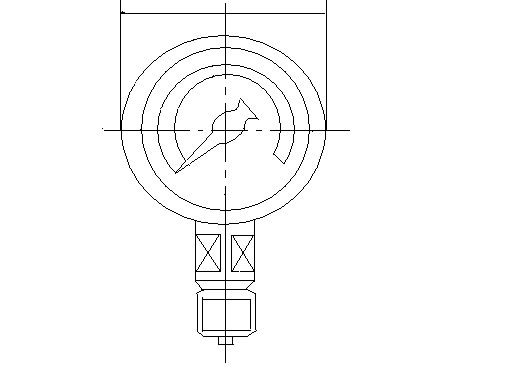
\includegraphics[width =0.45\textwidth]{figures/1.1.1.png}
    \caption{}
\end{figure}
\begin{figure}[!htbp]
    \centering
    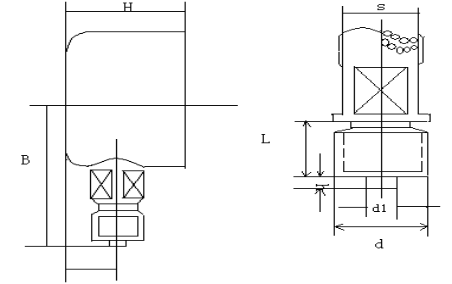
\includegraphics[width =0.65\textwidth]{figures/1.1.2.png}
    \caption{表壳外形尺寸}
    \label{figure1.1}
\end{figure}
\newline
接头位置为径向;表壳无边;表壳公称直径D=100mm;$H{\le}60mm$,
\begin{equation}
{B{\le}100mm,a=M20{\times}1.5,S=17_{-0.28}^{\circ},\\L=20_{{\pm}0.52},h=5_{{\pm}0.30},d_{1}=6_{-0.30}}\nonumber
\end{equation}
\subsection{标尺特性}
等分分度;标度角:$270^{\circ}$;
\begin{table}[!htbp]
    \centering
\caption{测量上限值与最小分度值的关系}
\label{tab:1.1}
    \begin{tabular}{|c|c|c|c|c|c|c|} \hline 
         测量上限值&0.06&0.1&0.16&0.25&0.4&0.6\\ \hline 
         测量下限值&0.001&0.002&0.005&0.005&0.01&0.01\\ \hline 
         测量上限值&1&1.6&2.5&4&0.6& \\ \hline 
         测量下限值&0.02&0.05&0.05&0.1&0.1& \\ \hline
    \end{tabular}
\end{table}
\newline

由\autoref{tab:1.1},由于我们设计的压力表量程上限为0.4Mpa,所以选择最小分度值为0.01.所以,所设计的压力表最小分度值为0.01MPa(${\approx}10kgf/cm^2$)

\section{方案论证}
\subsection{结构概述}
弹簧管压力表是一种用来测量气体压力的仪表。
\newline
压力表的组成:
\begin{itemize}
    \item 灵敏部分(弹簧管)
    \item 传动放大部分(曲柄滑块、齿轮机构)
    \item 示数部分(指针、刻度盘)
    \item 辅助部分(支承、轴、游丝)
\end{itemize}
\subsubsection{灵敏元件}
将不便测量的物理量转换成易于直接比较的物理量,本设计将弹簧管作为灵敏元件,将不易于比较的压力转换为易于测量的位移.
\subsubsection{传动放大机构}
本设计由曲柄滑块机构和齿轮传动机构组成.目的在于传递或放大位移,改变位移性质和得到等分刻度,并且应具有一定的补偿特性,同时仪表有较好的线性特性.
\subsubsection{示数装置}
其作用是在接受传动放大机构的位移后,指示出待测量的数值.本设计采用指针指示标尺刻度.
\subsection{原理分析}
作为灵敏元件的弹簧管可以把气体压力转变为管末端的位移,通过曲柄滑块机构将此位移转变为曲柄的转角,然后通过齿轮机构将曲柄转角放大,带动指针偏转,从而指示压力的大小。将转角放大便于测量,可以提高测量精度。压力表工作原理和框图如\autoref{FIGURE2.1}和\autoref{FIGURE2.2}所示。
\begin{figure}[!htbp]
    \centering
    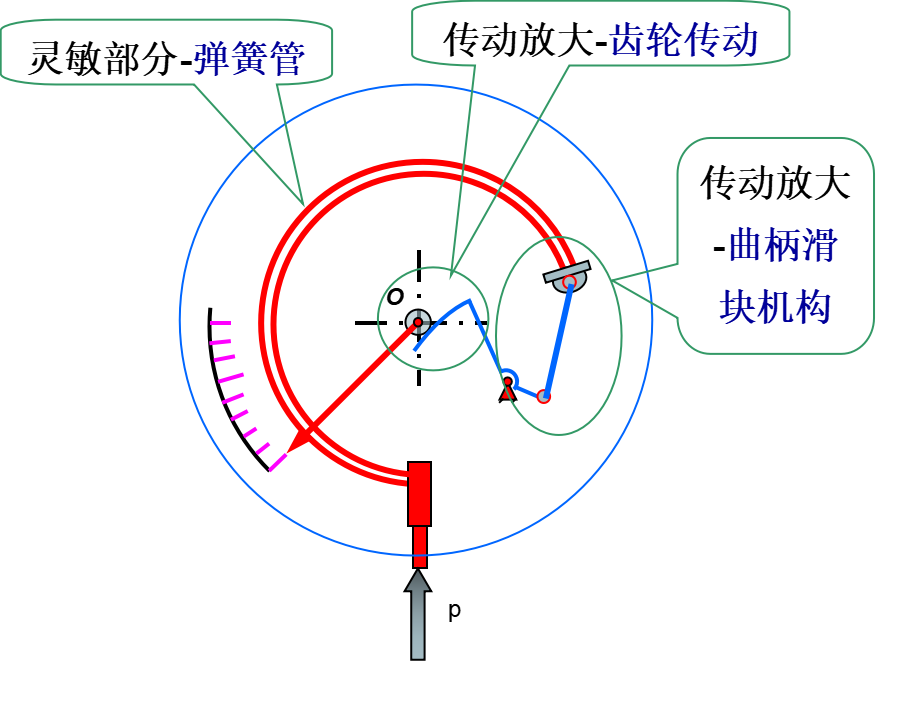
\includegraphics[width =0.5\textwidth]{figures/2.1.png}
    \caption{压力表工作原理}
    \label{FIGURE2.1}
\end{figure}
\begin{figure}[!htbp]
    \centering
    
\includegraphics[width =\textwidth]{figures/2.2.png}
    \caption{压力表工作原理框图}
    \label{FIGURE2.2}
\end{figure}
\newline

弹簧管的压力-位移是线性关系,但弹簧管本身的工艺问题(如材料、加工等)会造成一些线性误差,弹簧管形状的不直、不均匀也会导致非线性误差。曲柄滑块机构可以补偿弹簧管的线性及非线性误差。从$0{\sim}0.4Mpa$调整满足满刻度精度为线性误差调整,中间部分不均匀调整为非线性误差调整。

% \subsection{弹簧管}
% 将不便测量的物理量转换成易于直接比较的物理量,本设计将弹簧管作为灵敏元件,将不易于比较的压力转换为易于测量的位移.
% \subsection{曲柄滑块机构}
% 将弹簧管的非线性位移通过曲柄滑块机构转化成齿轮的线性转动。
% \subsection{齿轮传动}
% 通过设计两个齿轮的中心距,选定模数、小齿轮齿数,大齿轮的扇形角,大小齿轮的分度圆直径,尺顶圆直径,齿根圆直径来达到恒定传动比,将曲柄滑块的线性角度传动传动到指针转动的角度。
% \subsection{游丝}
% 游丝属于平面涡卷弹簧,它是由金属带材在一个平面内绕成的螺旋线形状的一种惯性元件,游丝工作时其外端固定在机壳上,内端固定在转轴上,随转轴一起旋转,游丝承受转矩而盘紧,放松时产生反作用力而工作,游丝在工作中时各圈之间是不接触的。游丝的功能是保持仪表传动系统单向接触,消除齿轮。铰销消除产生的回差。
% \subsection{标尺指针}

\section{参数选择}
\subsection{弹簧管}
\begin{tabular}{@{}>{\raggedright\arraybackslash}p{0.4\linewidth}>{\centering\arraybackslash}p{0.4\linewidth}@{}}
    毛坯外径 & $\phi = 15mm$ \\
    毛坯中径 & $R = 50mm$ \\
    壁厚 & $h = 0.3mm$ \\
    轴比 & $\frac{a}{b} = 4$ \\
    中心角 & $\gamma'' = 250°$ \\
    材料 & 锡青铜(QSn4-0.3) \\
    泊松比 & $\mu = 0.3$ \\
    弹性模量E & $1.127 \times 10^5MPa$
\end{tabular}
\newline

如\autoref{FIGURE3.1}所示:
\begin{figure}[!htbp]
    \centering
    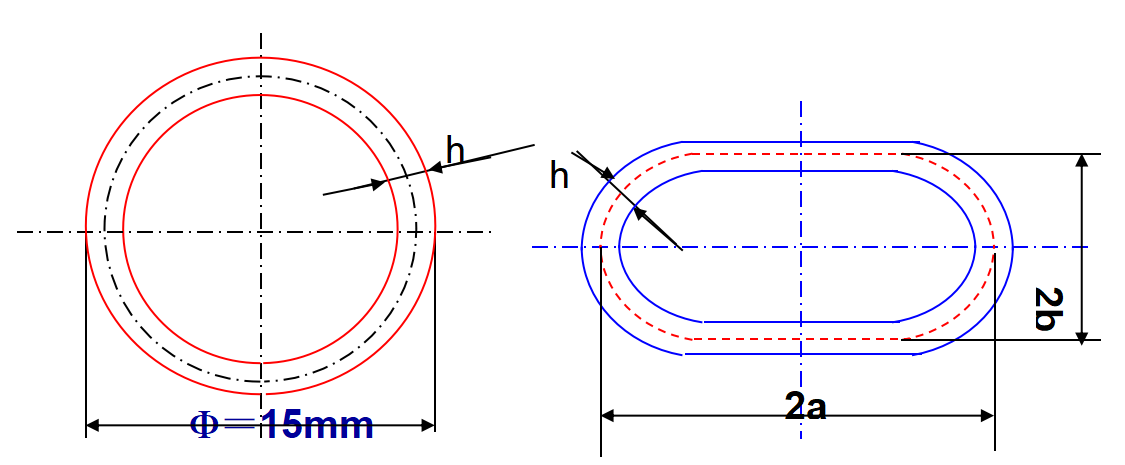
\includegraphics[width =\textwidth]{figures/3.1.png}
    \caption{弹簧管尺寸示意图}
    \label{FIGURE3.1}
\end{figure}
\subsection{曲柄滑块机构}
\begin{tabular}{@{}>{\raggedright\arraybackslash}p{0.4\linewidth}>{\raggedright\arraybackslash}p{0.4\linewidth}@{}}
相对杆长 : $\lambda=4$ &相对轴偏量 : $\varepsilon=1$\\
转动范围角 : $\alpha_p=18^\circ$ &初始位置角:$\alpha_0=-9^\circ$\\
终止位置角 : $\alpha_k=9^\circ$ &
\end{tabular}
\subsection{齿轮传动参数的选择}
\begin{tabular}{@{}>{\raggedright\arraybackslash}p{0.4\linewidth}>{\raggedright\arraybackslash}p{0.4\linewidth}@{}}
模数 : $m=0.25$ &小齿轮齿数 : $z_2=21$\\
传动比 : $i_{21}=15$& 
\end{tabular}
\subsection{标尺指针参数选择}
\begin{tabular}{@{}>{\raggedright\arraybackslash}p{0.4\linewidth}>{\raggedright\arraybackslash}p{0.4\linewidth}@{}}
分度尺寸:$3.375^{\circ}$ & 短标线长度:5mm\\
长标线长度:10mm & 指针与短标线重合长度:2mm\\
指针形状:楔杆形& 指针末端宽度:2mm
\end{tabular}
\subsection{游丝的选择}
\begin{tabular}{@{}>{\raggedright\arraybackslash}p{0.4\linewidth}>{\raggedright\arraybackslash}p{0.4\linewidth}@{}}
外径:$D_1=25mm$ & 内径:$D_2=5mm$\\
圈数:$n=10$ & 安装角度:$\phi_{min}=\frac{\pi}{2}$\\
宽度比:$\eta=6$ & 摩擦系数:$f=0.2$\\
当量摩擦系数:$f_v=0.314$ & 
\end{tabular}
\section{参数计算}
\subsection{弹簧管有关参数的确定}
\subsubsection{弹簧管外型参数的确定}
单位:(mm)
\begin{center}
\begin{tabular}{|>{\centering\arraybackslash}p{0.3\linewidth}|>{\centering\arraybackslash}p{0.3\linewidth}|>{\centering\arraybackslash}p{0.3\linewidth}|}
\hline
项目 & 公式依据 & 计算结果 \\
\hline
$x(2b=x,2a=4x)$ & $\pi(\phi-h)=\pi x+2(4x-x)$ & 5.050 \\
\hline
短轴中径$2b$ & $2b=x$ & 5.050 \\
\hline
长轴中径$2a$ & $2a=4x$ & 20.200 \\
\hline
短轴$2B$ & $2B=2b+h$ & 5.350 \\
\hline
长轴$2A$ & $2A=2a+h$ & 20.500 \\
\hline
\end{tabular}
\end{center}
\subsubsection{弹簧管末端位移的确定}
\begin{center}
\begin{tabular}{|>{\centering\arraybackslash}p{0.2\linewidth}|>{\raggedright\arraybackslash}p{0.5\linewidth}|>{\centering\arraybackslash}p{0.2\linewidth}|}
\hline
项目 & \multicolumn{1}{|c|}{公式依据} & 计算结果 \\
\hline
$\frac{\gamma-\gamma'}{\gamma}$ & $(1)\frac{\gamma-\gamma'}{\gamma}=p\frac{1-{\mu}^2}{E}\frac{R^2C_1}{bh[C_2+(\frac{Rh}{a^2})^2]}(1-\frac{b^2}{a^2})$ & $1.225\times10^{-2}$ \\
\hline
径向位移$S_r$ & $(2)S_r=\frac{\gamma-\gamma'}{\gamma}R(1-cos\gamma)$ & 1.046mm \\
\hline
切向位移$S_t$ & $(3)S_t=\frac{\gamma-\gamma'}{\gamma}R(\gamma-sin\gamma)$ & 2.837mm \\
\hline
总位移$S$ & $(4)S=\sqrt{S_r^2+S_t^2}$ & 3.024mm \\
\hline
位移方向角$\phi$ & $(5)\phi=arctan\frac{S_r}{S_t}$ & $20.24^{\circ}$ \\
\hline
\end{tabular}
\end{center}
附:查表$C_1=0.437,C_2=0.121,\gamma=225^\circ$
\subsection{曲柄滑块机构参数的确定}
\begin{figure}[!htbp]
    \centering
    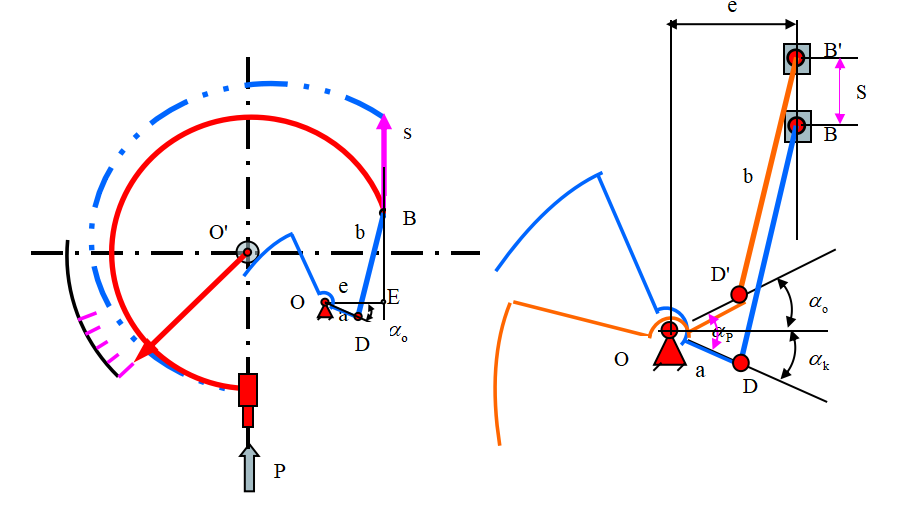
\includegraphics[width =\textwidth]{figures/4.2.1.png}
    \caption{曲柄滑块结构简图}
    \label{FIGURE4.2.1}
\end{figure}
\begin{figure}[!htbp]
    \centering
    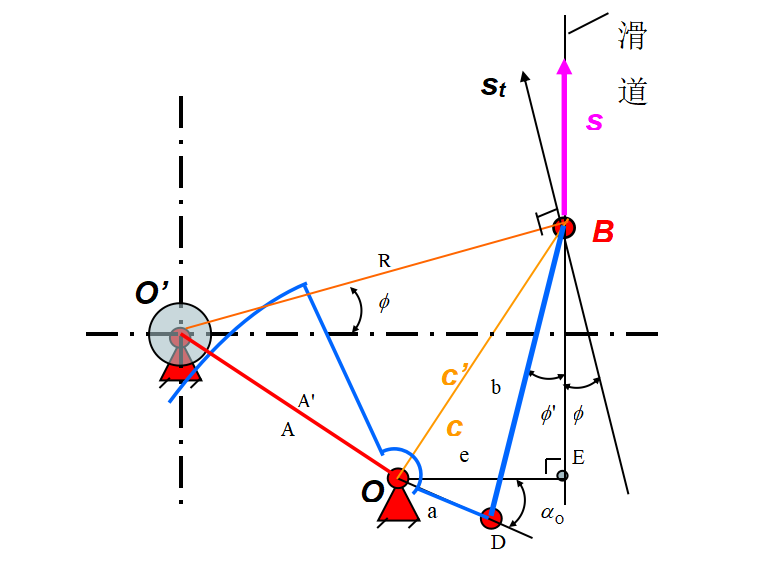
\includegraphics[width =\textwidth]{figures/4.2.2.png}
    \caption{中心距计算图}
    \label{FIGURE4.2.2}
\end{figure}
\begin{center}
\begin{tabular}{|>{\centering\arraybackslash}p{0.1\linewidth}|>{\centering\arraybackslash}p{0.7\linewidth}|>{\centering\arraybackslash}p{0.1\linewidth}|}
\hline
项目 & 公式依据 & 计算结果 \\
\hline
曲柄长度 $a$& \(\displaystyle a = \frac{s}{(\sin\alpha_k - \sin\alpha_o)+\sqrt{\lambda^2 - (\cos\alpha_o - {\varepsilon})^2}-\sqrt{\lambda^2 - (\cos\alpha_k - {\varepsilon})^2}}\)& \(9.665\)mm\\\hline
连杆初算值 $b'$& \(b' = a\lambda\)& \(38.662\)mm\\
\hline
偏移距 $e$ & \(e = a\varepsilon\) & \(9.665\)mm \\
\hline
连杆初始位与滑块运动夹角 $\phi'$ & \(\phi' = \arcsin\frac{a\cos\alpha_k - e}{b'}\) & \(-0.176^\circ\) \\
\hline
$\alpha_5$& \(\alpha_5 = 90^\circ - \alpha_k + \phi'\) & \(80.824^\circ\) \\
\hline
$c'$ & \(c' = \sqrt{a^2 + (b')^2 - 2ab'\cos\alpha_5}\) & \(38.327\)mm \\
\hline
$\alpha_7$ & \(\alpha_7 = 90^\circ - \phi - \sin^{-1}\frac{e}{c'}\) & \(55.154^\circ\) \\
\hline
理论中心距 $A'$ & \(A' = \sqrt{R^2 + (c')^2 - 2Rc'\cos\alpha_7}\) & \(42.178\)mm \\
\hline
实际中心距 $A$ & (6){\qquad}\( A = \frac{mz_2}{2}(i_{21} + 1)\)& \(42.000\)mm \\
\hline
$\alpha_9$ & \(\alpha_9 = \arccos\frac{R\cos\phi - e}{A} + \phi\) & \(47.760^\circ\) \\
\hline
修正后 $c$ & \(c = \sqrt{A^2 + R^2 - 2AR\cos\alpha_9}\) & 37.955mm\\
\hline
修正后 $b$ & \(b = \sqrt{a^2 + c^2 - 2ac\cos(\alpha_o + \alpha_7 + \phi)}\) & \(35.216\)mm \\
\hline
扇形角 $V_\text{齿}$& \(V_\text{齿} = \alpha_p(1 + 25\%) + 2\)个齿的度数& \(27.070^\circ\) \\ \hline
\end{tabular}
\end{center}
\subsection{压力表原理误差分析}
\begin{equation}
S_n = \frac{\alpha_n - \alpha_o}{\alpha_k - \alpha_o} S
\end{equation}
\begin{equation}
(7) {\quad S_n' = a(\sin\alpha_n - \sin\alpha_o) + a\sqrt{\lambda^2 - (\cos\alpha_o - \varepsilon)^2} - a\sqrt{\lambda^2 - (\cos\alpha_n - \varepsilon)^2}}
\end{equation}
\begin{center}
    \begin{tabular}{|>{\centering\arraybackslash}p{0.1\linewidth}|>{\centering\arraybackslash}p{0.15\linewidth}|>{\centering\arraybackslash}p{0.15\linewidth}|>{\centering\arraybackslash}p{0.2\linewidth}|>{\centering\arraybackslash}p{0.2\linewidth}|}
        \hline
         $\alpha_n$ & 理想值 $S_n$ & 实际值 $S_n'$ & 原理误差绝对值$|S_n-S_{n}'|$& 原理误差相对值$|S_n-S_{n}'|/S_n$\\
         \hline
         $9^\circ$ & 3.1400& 3.1406 & 0.0006 & 0.0184\% \\
         \hline
         $7^\circ$ & 2.7911 & 2.7935 & 0.0024 & 0.0853\% \\
         \hline
         $5^\circ$ & 2.4423 & 2.4450 & 0.0028 & 0.1132\% \\
         \hline
         $3^\circ$ & 2.0933 & 2.0954 & 0.0021 & 0.1011\% \\
         \hline
         $1^\circ$ & 1.7444 & 1.7453 & 0.0008 & 0.0483\% \\
         \hline
         $-1^\circ$ & 1.3956 & 1.3949 & 0.0006 & 0.0461\% \\
         \hline
         $-3^\circ$ & 1.0465 & 1.0448 & 0.0019 & 0.1828\% \\
         \hline
         $-5^\circ$ & 0.6986 & 0.6952 & 0.0026 & 0.3626\% \\
         \hline
         $-7^\circ$ & 0.3489 & 0.3468 & 0.0020 & 0.5861\% \\
         \hline
         $-9^\circ$ & 0 & 0 & 0 & 0 \\
         \hline
    \end{tabular}
\end{center}
\subsection{游丝应力校核}
% Please add the following required packages to your document preamble:
% \usepackage{multirow}
\begin{center}
\begin{tabular}{|>{\centering\arraybackslash}p{0.07\linewidth}|>{\centering\arraybackslash}p{0.06\linewidth}|>{\centering\arraybackslash}p{0.5\linewidth}|>{\centering\arraybackslash}p{0.2\linewidth}|}
\hline
\multicolumn{2}{|c|}{项目}& 公式依据 & 计算结果 \\ \hline
\multicolumn{2}{|c|}{$P_1$}& \(P_1=m_\text{轴}+m_\text{帽}+m_\text{游丝}+m_\text{指针},m=\rho vg\)&$0.063N$\\ \hline
\multicolumn{2}{|c|}{$P_2$}& $P_2=m_\text{扇形齿轮}+m_\text{齿轮中心轴}$ & $0.050N$ \\ \hline
\multirow{3}{*}{竖直放}&$Mf_{z1}$& \(Mf_{z1}=\frac{1}{2}f_v P_1 d, f_v =0.2,\,f=0.314\)& $1.73\times10^{-5}Nm$ \\ \cline{2-3} 
 &$Mf_{z2}$&  $Mf_{z2}=\frac{1}{2}f _vP_2 d$& $1.62\times10^{-5}Nm$ \\ \cline{2-3}
 &$Mf_z$& $Mf_z =Mf_{z1}+Mf_{z2}\frac{1}{i}\frac{1}{\eta}(\eta=0.9) $& $2.12\times10^{-5}Nm$ \\ \hline
\multirow{3}{*}{水平放}&$Mf_{z1}$& $Mf_{z1}=\frac{1}{3}P_1 f \frac{d_1^3-d_2^3}{d_1^2-d_2^2} ,d_1=1.1d_2, f=0.2 $& $1.17\times10^{-5}Nm$ \\ \cline{2-3}
 &$Mf_{z2}$&  $Mf_{z2}=\frac{1}{3}P_2 f \frac{d_1^3-d_2^3}{d_1^2-d_2^2}$& $1.02\times10^{-5}Nm$ \\ \cline{2-3}
 &$Mf_z$& $Mf_z =Mf_{z1}+Mf_{z2}\frac{1}{i_{\textit{齿}21}}\frac{1}{\eta_{21}}  $& $2.23\times10^{-5}Nm$ \\ \hline
\multicolumn{2}{|c|}{$\max(Mf_z)$}& $\max(Mf_z\textit{竖直}, Mf_z\textit{水平})$& $2.23\times10^{-5}Nm$ \\ \hline
\multicolumn{2}{|c|}{$M_{min}$}& $(8)\quad M_{min}=\frac{kMf_z}{1-k\xi},k=2.5,\xi=0.1$ & $7.45\times10^{-5}Nm$ \\ \hline 
\multicolumn{2}{|c|}{$M_{\text{max}}$}& $M_{\text{max}}=M_{\text{min}}\frac{{\phi}_{max}}{{\phi}_{min}}=4M_{\text{min}}$& $3.21\times10^{-4}\, \text{Nm}$ \\
\hline
\multicolumn{2}{|c|}{初定游丝长$L$}& $(9){\quad }L=\pi n\frac{D_1+D_2}{2}$& $574.5\, \text{mm}$ \\
\hline
\multicolumn{2}{|c|}{初定游丝厚$h$}& $(10){\quad }h=\sqrt[4]{\frac{12LM_{\text{min}}}{\mu E \phi_{\text{min}}}},\,E = 1.1 \times 10^5 \text{MPa} $& $0.28\, \text{mm}$\\
\hline
\multicolumn{2}{|c|}{初定游丝宽$b$}& $(11){\quad }b = \mu h$& $1.61\, \text{mm}$\\
\hline
\multicolumn{2}{|c|}{最大应力$\sigma_{\text{max}}$}& $(12){\quad }\sigma_{\text{max}}=\frac{6M_{\text{max}}}{bh^2}$& $194.7\, \text{MPa}$\\
\hline
\multicolumn{2}{|c|}{许用应力$[\sigma_{b}]$}& $[\sigma_{b}]=\frac{\sigma_{b}}{s},\,s = 3.2,\, \sigma_{b} = 640\, \text{MPa}$& $200\, \text{MPa}$\\
\hline
\end{tabular}
\end{center}
结论:因为${\sigma}_{max}<{\sigma}_{b}$,因此各参数选择计算合理。
\subsection{游丝系数确定}
注意:式子中K为游丝个数。在实际加工之后游丝的a、D1、D2有微小改变,但并不影响游丝的特性,故可得出在实际加工之后a、D1、D2不必再根据K值重新计算;\\
由4.4可得游丝基本参数:\\
\begin{tabular}{@{}>{\centering\arraybackslash}p{0.3\linewidth}>{\centering\arraybackslash}p{0.3\linewidth}@{}}
    游丝长度L & 574.5 \\
    游丝圈数n & 9 \\
    圈间距a & 1.5 \\
    游丝个数K & 4
\end{tabular}
\begin{center}
\begin{tabular}{|>{\centering\arraybackslash}p{0.25\linewidth}|>{\centering\arraybackslash}p{0.3\linewidth}|>{\centering\arraybackslash}p{0.25\linewidth}|}
\hline
项目 & 公式依据 & 计算结果 \\ \hline
游丝长度 L & $(13)~L = \frac{Ebh^3\phi_{\text{min}}}{12M_{\text{min}}}$ & 574.5 \\ \hline
游丝圈数 n & $(14)~n = \frac{2L}{\pi(D_1 + D_2)}$ & 9 \\ \hline
圈间距 a & $(15)~a = \frac{D_1 - D_2}{2n}$ & 1.5mm \\ \hline
游丝个数 k & $(16)~k = \frac{a}{h}$ ($k \geq 3$) & 4个 \\ \hline
\end{tabular}
\end{center}
\section{设计总结}
压力表是工业常用的测量气体压力的仪器,在工业生产中具有举足重轻的作用.在实际生产中对压力表的要求非常严格,要求有足够的精度,灵敏度,并要求安全可靠.同时根据不同的工作任务和条件,对压力表提出特殊要求,如耐高温,抗震,防潮,防尘等.
\newline

本设计要求为普通工业气体压力表,我们的设计方案为弹簧管压力表,它具有灵敏度高,造价低廉,结构简单,传动平稳,易于加工和制造及适应性强等特点,经过以上设计和计算表明,该方案基本达到了设计要求,完成了规定的设计任务.
\newline

同时,本设计也存在一些不足,对工作环境及测量气体均无具体要求,没有考虑它们对压力表的影响.另外,环境的温度,湿度及气体对压力表的腐蚀都可能降低其精密度.
\newline

在近三周的课程设计中,我将机械零件与制图等课程有机结合起来,提高了自己的综合能力和独立完成工作的能力,并初步掌握了机械仪表的设计方法和初步树立正确的设计思想.
\newline

工作过程中,我受到了指导老师和同学们的大力支持和帮助,在此深表感谢.
\section{标准化统计}
\begin{center}
\begin{tabular}{|>{\centering\arraybackslash}p{0.2\linewidth}|>{\centering\arraybackslash}p{0.2\linewidth}|>{\centering\arraybackslash}p{0.2\linewidth}|>{\centering\arraybackslash}p{0.2\linewidth}|}
\hline
国标代号 & 零件名称 & 数量 & 材料\\ \hline
GB65-02 & 螺钉 M2 & 3 & H62\\ \hline
GB65-02 & 螺钉 M3 & 4 & H62\\ \hline
GB948-02 & 螺钉 M5 & 4 & HPb59-1\\ \hline
GB97-02 & 垫圈 2 & 4 & GB97-02\\ \hline
GB97-02 & 垫圈 3 & 1 & GB97-02\\ \hline
GB117-02 & 圆柱销 & 1 & HPb59-1Y\\ \hline
\end{tabular}
\end{center}
\begin{itemize}
    \item 标准件总数:17
    \item 零件总数:45   
    \item 标准化率:37.7\%
\end{itemize}     
   

\section{公式来源}
附表:
\begin{center}
\begin{tabular}{|>{\centering\arraybackslash}p{0.2\linewidth}|>{\centering\arraybackslash}p{0.4\linewidth}|>{\centering\arraybackslash}p{0.2\linewidth}|} \hline
\textit{公式代号}& \textit{参考书名称} & \textit{页数} \\ \hline
(1) &  & $P_{45}$ 2-51\\ \cline{1-1}\cline{3-3}
(2) & \textit{《精密机械零件》}& $P_{ 46}$ 2-52\\ \cline{1-1}\cline{3-3}
(3) &\textit{天津大学} & $P_{ 46}$ 2-53\\ \cline{1-1}\cline{3-3}
(4) & \textit{庞振基 ,\,傅雄刚主编}  & $P_{ 46}$ 2-54\\ \cline{1-1}\cline{3-3}
(5) &  & $P_{ 46}$ 2-55\\ \hline
(6) & \textit{《精密机械设计》} & $P_{ 222}$ 8-94\\ \cline{1-1}\cline{3-3}
(7) & \textit{庞振基 ,\,黄其圣主编} & $P_{ 90}$ 5-12\\ \hline
(8) & \textit{《仪表零件及机构》} & $P_{ 177}$ 7-44\\ \hline
(9) & & $P_{ 347}$  13-22\\ \cline{1-1}\cline{3-3}
(10) &  & $P_{ 347}$ 13-24\\ \cline{1-1}\cline{3-3}
(11) &  & $P_{ 347}$ 13-25\\ \cline{1-1}\cline{3-3}
(12) & \textit{《精密机械设计》}  & $P_{ 347}$ 13-26\\ \cline{1-1}\cline{3-3}
(13) & \textit{庞振基,\,黄其圣主编}& $P_{ 346}$ 13-21\\ \cline{1-1}\cline{3-3}
(14) &  & $P_{ 347}$ 13-22\\ \cline{1-1}\cline{3-3}
(15) & & $P_{ 348}$ 13-27\\ \cline{1-1}\cline{3-3}
(16) & & $P_{ 348}$ 13-28\\ \hline
\end{tabular}
\end{center}


%%------------------------------参考文献---------------------------%%
\newpage
\reference
\addcontentsline{toc}{section}{参考文献}   % 将参考文献作为一级标题加入到目录

\end{document}